\documentclass[pdf]{beamer}
\usepackage[utf8]{inputenc}
\usepackage{graphicx}
\usepackage[T1]{fontenc}      
\usepackage[francais]{babel}
\usepackage{graphicx}
\usepackage{circuitikz}
\usepackage[squaren, Gray]{SIunits}
\usepackage{sistyle}
\usepackage[autolanguage]{numprint}
\usepackage{pgfplots}
\usepackage{amsmath,amssymb,array}

\usetheme{warsaw}
\mode<presentation>{}

\title{Projet 2 : concevoir un haut-parleur}
\subtitle{Pré-jury}
\author{Groupe 115.3}
\date{13 mars 2014}

\begin{document}

% =======================================================================
\begin{frame}
	\titlepage
\end{frame}

% =======================================================================
\begin{frame}
	\frametitle{Etat d'avancement du projet}	

	\begin{itemize}
		\item Recherches documentaires (distorsion harmonique et contre-réaction négative) ;
		\item Analyse des filtres passe-haut/passe-bas ;
		\item Dimensions de la bobine et membrane ;
		\item Cahier des charges ;
		\item Soudure d'une plaquette.
	\end{itemize}

	\underline{Le planning}
	\begin{itemize}
		\item S8 : bobiner et souder 2ème plaque ;
		\item S9 : finaliser la membrane et la tester ;
		\item S10 : réaliser le caisson du haut-parleur ;
		\item S11 : fabriquer le 2ème haut-parleur ;
		\item S12 - S13 : rédaction du rapport final ;
		\item S14 : préparation de ladéfense orale.
	\end{itemize}
\end{frame}

% =======================================================================
\begin{frame}
	\frametitle{Recherche documentaire}
	\framesubtitle{La contre-réaction (ou contre réaction négative)}
	
	\textbf{Principe} : réinjection d'une partie du signal de sortie à l'entrée.
	
	\begin{columns}
		\begin{column}{5cm}
			\includegraphics{opamp_loop.png}
		\end{column}
		
		\begin{column}{5cm}
				\begin{itemize}
					\item Signal de sortie plus proche du signal d'entrée ;
					\item	Réduction des signaux parasites et de la distorsion ;
					\item Contrôle du gain ;
					\item Elargissement de la bance passante ;
					\item Réducion de l'impédance de sortie.
				\end{itemize}
		\end{column}
	\end{columns}
\end{frame}

% =======================================================================
\begin{frame}
	\frametitle{Recherche documentaire}
	\framesubtitle{La distorsion}
	
	\textbf{Principe} : des fréquences harmoniques s'ajoutent à la fréquence fondamentale
	$\Rightarrow$ modification du signal.
	
	\bigbreak
	
	\begin{columns}
		\begin{column}{5cm}
			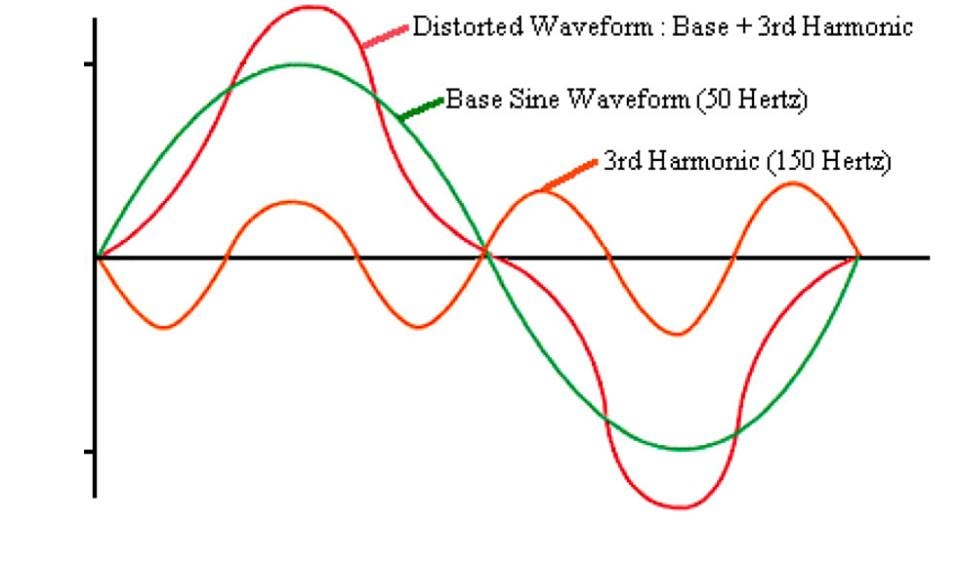
\includegraphics[scale=0.17]{distorsion.jpg}
		\end{column}
		
		\begin{column}{5cm}
			\begin{itemize}
				\item	Filtres actifs ou passifs (passe-haut et passe-bas) ;
				\item Boucle de contre-réaction (réduction du TDH de 1\% à 0.001\%).
			\end{itemize}
		\end{column}
	\end{columns}

\end{frame}
	
% =======================================================================
\begin{frame}
	\frametitle{Approximation de la fréquence de coupure}
	\framesubtitle{Passe-bas}

	\begin{center}
		\begin{array}{rcel}
			$$
			\begin{pmatrix}  
				4.204 & 1\\
				4.255 & 1 \\
				4.301 & 1 
			\end{pmatrix} &

			\begin{pmatrix}  
				a\\
				b
			\end{pmatrix} &

			= &

			\begin{pmatrix}  
				1.7\\
				1.55\\
				1.45
			\end{pmatrix}
			$$
		\end{array}
	\end{center}	

	$$\fbox{y_H = 0.75, y_D = -1.96 \cdot \log(x) + 9.84}$$

	$$\fbox{x = 5557.7 Hz}$$ 

	Pour une résistance totale de $\unit{57.5}{\ohm}$ et une capacité de \unit{470 \cdot 10^{-9}}{\farad} on a :

	\begin{center}
		\includegraphics[scale=0.5]{cutoff_f1.png}  
	\end{center}
	
\end{frame}

% =======================================================================
\begin{frame}
	\frametitle{Approximation de la fréquence de coupure}
	\framesubtitle{Passe-haut}
	
	\begin{center}
		\begin{array}{rcel}
			$$
			\begin{pmatrix}  
				2.1 & 1\\
				2.3 & 1 \\
				2.6 & 1 
			\end{pmatrix} &

			\begin{pmatrix}  
				a\\
				b
			\end{pmatrix} &

			= &

			\begin{pmatrix}  
				0.4\\
				0.5\\
				0.6
			\end{pmatrix}
			$$
		\end{array}
	\end{center}

	$$\fbox{y_H = 0.75, y_D = 0.7 \cdot \log(x) -1.11}$$

	$$\fbox{x = 439.4 Hz}$$ 

	Pour une resistance totale de $\unit{57.5}{\ohm}$ et une capacité de $\unit{470 \cdot 10^{-9}}{\farad}$ on a :

	\begin{center}
		\includegraphics[scale=0.5]{cutoff_f2.png}  
	\end{center}
	
\end{frame}

% =======================================================================
\begin{frame}
	\frametitle{Modélisation du filtre passe-bas}

	\begin{columns}
		\begin{column}{5cm}
			\scalebox{0.5}{\includegraphics{lwp_voltages.png}}
		\end{column}
		
		\begin{column}{5cm}
			\begin{itemize}
				\item $V_{out}$ est en retard de $\arctan{RC\omega}$ par rapport à $V_{in}$ ;
				\item Le déphasage augmente avec la fréquence.
			\end{itemize}
		\end{column}
	\end{columns}
	
	\begin{columns}
		\begin{column}{5cm}
			\begin{itemize}
				\item Atténue les hautes fréquences ;
				\item Laisse passer les basses fréquences.
			\end{itemize}
		\end{column}

		\begin{column}{5cm}
			\scalebox{0.5}{\includegraphics{lwp_ratio.png}}
		\end{column}
	\end{columns}
\end{frame}

% =======================================================================
\begin{frame}
	\frametitle{Modélisation du filtre passe-haut}
	
	\begin{columns}
		\begin{column}{5cm}
			\scalebox{0.5}{\includegraphics{hgp_voltages.png}}
		\end{column}
		
		\begin{column}{5cm}
			\begin{itemize}
				\item $V_{out}$ est en retard de $\arctan{RC\omega}$ par rapport à $V_{in}$ ;
				\item Le déphasage augmente avec la fréquence.
			\end{itemize}
		\end{column}
	\end{columns}
	
	\begin{columns}
		\begin{column}{5cm}
			\begin{itemize}
				\item Atténue les basses fréquences ;
				\item Laisse passer les hautes fréquences.
			\end{itemize}
		\end{column}

		\begin{column}{5cm}
			\scalebox{0.5}
			{\includegraphics{hgp_ratio.png}}
		\end{column}
	\end{columns}
\end{frame}

% =======================================================================
\begin{frame}
	\frametitle{Dimensionnement du haut-parleur}
	
	\begin{columns}
		\begin{column}{5cm}
			\scalebox{0.3}{\includegraphics{baffle.png}}
		\end{column}
		
		\begin{column}{5cm}
				\begin{itemize}
					\item Boite cubique de $\unit{0.30}{\meter}$ de côté ;
					\item Membrane de $\unit{0.16}{\meter}$ de diamètre $\unit{0.06}{\meter}$ de profondeur ;	
					\item Papier carton de $\unit{0.200}{\kilogram\per\meter^2}$.
				\end{itemize}
		\end{column}
	\end{columns}
	
\end{frame}

% =======================================================================
\begin{frame}
	\frametitle{Dimensionnement des bobines}

	\begin{columns}
		\begin{column}{5cm}
			\scalebox{0.2}{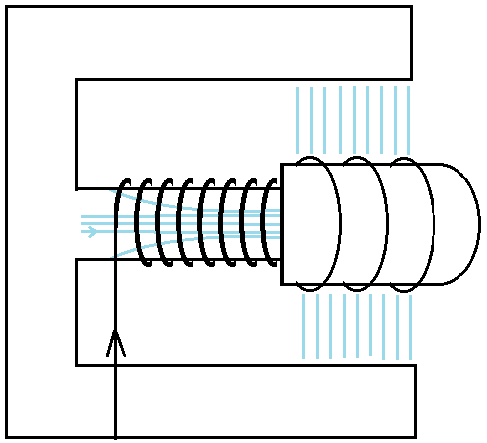
\includegraphics{hautparleur.png}}
		\end{column}
		
		\begin{column}{5cm}
			La bobine fixe joue un rôle d'électroaimant. Dans des conditions idéales, le champ total crée est $B = \unit{0.1143}{\tesla}$.
		\end{column}
	\end{columns}

	\bigbreak

	\paragraph{\textbf{Tableau récapitulatif}}
	\small
	{
		\begin{center}
		\begin{tabular}{c|c|c|c|c|c}
			$$ & $N$ & $I$ & $R$ & $L$ & $L_{fil}$ \\
			\hline
			Bobine fixe & $400$ & $\unit{2.5}{\ampere}$ & \unit{7.254}{\ohm} & $\unit{0.01475}{\henry}$ & $\unit{40.3}{\meter}$ \\
			\hline
			Bobine mobile & $ 118 $ & $\unit{0.1667}{\ampere}$ & $\unit{2.38}{\ohm}$ & $\unit{0.0734}{\henry}$ & $\unit{12.6}{\meter}$ \\
		\end{tabular}
		\end{center}
	}
\end{frame}
\end{document}